\documentclass[aspectratio=169,11pt]{beamer}

\usepackage[utf8]{inputenc}
\usepackage[T1]{fontenc}
\usepackage[brazil]{babel}
\usepackage{graphicx}
\usepackage{tikz}
\usetikzlibrary{calc,positioning}

\definecolor{bg}{RGB}{236,242,248}
\definecolor{ink}{RGB}{16,36,66}
\definecolor{muted}{RGB}{78,98,122}
\definecolor{card}{RGB}{255,255,255}
\definecolor{resnet}{RGB}{29,92,214}
\definecolor{efficient}{RGB}{12,138,125}
\definecolor{vit}{RGB}{112,52,196}
\definecolor{good}{RGB}{21,148,94}
\definecolor{mid}{RGB}{214,126,18}
\definecolor{bad}{RGB}{196,54,64}
\definecolor{soft}{RGB}{223,232,243}

\setbeamercolor{normal text}{fg=ink,bg=bg}
\setbeamercolor{frametitle}{fg=white,bg=ink}
\setbeamercolor{structure}{fg=resnet}
\setbeamerfont{frametitle}{series=\bfseries,size=\Large}
\setbeamertemplate{navigation symbols}{}
\setbeamertemplate{itemize item}{\textcolor{resnet}{\textbullet}}

\setbeamertemplate{background}{%
    \begin{tikzpicture}[remember picture,overlay]
        \fill[bg] (current page.north west) rectangle (current page.south east);
        \fill[resnet] (current page.north west) rectangle ([xshift=7pt]current page.south west);
    \end{tikzpicture}%
}

\setbeamertemplate{frametitle}{%
    \nointerlineskip
    \begin{beamercolorbox}[wd=\paperwidth,ht=14mm,dp=3mm,leftskip=8mm,rightskip=6mm]{frametitle}
        \insertframetitle
    \end{beamercolorbox}%
}

\setbeamertemplate{footline}{%
    \begin{beamercolorbox}[wd=\paperwidth,ht=6.5mm,dp=2mm,leftskip=8mm,rightskip=6mm]{frametitle}
        \scriptsize João \quad Wesley \quad André \hfill \insertframenumber\,/\,\inserttotalframenumber
    \end{beamercolorbox}%
}

\newcommand{\pill}[2]{%
    \tikz[baseline=-0.6ex]\node[rounded corners=8pt,fill=#1,text=white,inner xsep=8pt,inner ysep=3pt,font=\scriptsize\bfseries] {#2};%
}

\title{Classificadores ImageNet}
\subtitle{Vídeo gravado e webcam}
\author{João \and Wesley \and André}
\date{Outubro de 2026}

\begin{document}

\begin{frame}[plain]
    \begin{tikzpicture}[remember picture,overlay]
        \fill[ink] (current page.north west) rectangle ([xshift=0.34\paperwidth]current page.south west);
        \fill[resnet] ([xshift=0.34\paperwidth]current page.north west) rectangle ([xshift=0.355\paperwidth]current page.south west);
        \node[anchor=west, text=white, align=left, text width=0.28\paperwidth] at ([xshift=8mm,yshift=8mm]current page.west)
            {\scriptsize\textcolor{resnet}{\textbf{ETAPA 1}}\\[8pt]
             \Large\bfseries Vídeo\\e webcam\\[8pt]
             \scriptsize 3 redes prontas,\\sem treinamento novo.\\[8pt]
             João\\Wesley\\André};
        \node[anchor=north west, text=ink, align=left] at ([xshift=0.40\paperwidth,yshift=-16mm]current page.north west)
            {\Huge\bfseries Qual modelo\\acerta e qual\\responde a tempo?};
        \node[anchor=south west, align=left] at ([xshift=0.40\paperwidth,yshift=16mm]current page.south west) {%
            \pill{resnet}{ResNet-50}\hspace{4pt}%
            \pill{efficient}{EfficientNet-B0}\hspace{4pt}%
            \pill{vit}{ViT-B/16}\\[8pt]
            {\color{muted}\small ImageNet \quad\textbullet\quad CPU \quad\textbullet\quad 17 minutos}};
    \end{tikzpicture}
\end{frame}

\begin{frame}{Quatro paradas}
    \begin{center}
    \begin{tikzpicture}
        \foreach \x/\cor/\num/\titulo/\detalhe in {
            0/resnet/01/Olhar/{1.000 classes.\\Uma decisão por quadro.},
            1/efficient/02/Modelos/{ResNet, EfficientNet e ViT.\\Pesos e transforms oficiais.},
            2/vit/03/Teste/{Vídeo com rótulo.\\Webcam só com tempo.},
            3/mid/04/Escolha/{Top-1, top-5 e FPS.\\Tudo medido na CPU.}
        }{
            \fill[black!8, rounded corners=12pt] ({\x*3.15+0.06},-0.06) rectangle ({\x*3.15+2.95},3.55);
            \fill[card, rounded corners=12pt] ({\x*3.15},0) rectangle ({\x*3.15+2.9},3.6);
            \fill[\cor, rounded corners=12pt] ({\x*3.15+0.22},2.35) rectangle ({\x*3.15+1.35},3.15);
            \node[text=white, font=\bfseries] at ({\x*3.15+0.78},2.75) {\num};
            \node[anchor=north west, text=ink, font=\bfseries\large, align=left] at ({\x*3.15+0.22},2.05) {\titulo};
            \node[anchor=north west, text=muted, font=\small, align=left, text width=2.45cm] at ({\x*3.15+0.22},1.55) {\detalhe};
        }
    \end{tikzpicture}
    \end{center}
\end{frame}

\begin{frame}{A mesma cena, duas perguntas}
    \begin{center}
    \begin{tikzpicture}
        \fill[black!8, rounded corners=14pt] (0.08,-0.08) rectangle (6.15,4.35);
        \fill[card, rounded corners=14pt] (0,0) rectangle (6.05,4.45);
        \fill[resnet, rounded corners=14pt] (0,3.75) rectangle (6.05,4.45);
        \node[text=white, font=\bfseries] at (3.02,4.1) {Vídeo gravado};
        \node[align=center, text=ink] at (3.02,2.15)
            {\Huge 56\%?\\[4pt]{\large\color{muted} a classe principal\\está correta?}};

        \fill[black!8, rounded corners=14pt] (6.55,-0.08) rectangle (12.7,4.35);
        \fill[card, rounded corners=14pt] (6.45,0) rectangle (12.6,4.45);
        \fill[efficient, rounded corners=14pt] (6.45,3.75) rectangle (12.6,4.45);
        \node[text=white, font=\bfseries] at (9.52,4.1) {Webcam};
        \node[align=center, text=ink] at (9.52,2.15)
            {\Huge 25 FPS?\\[4pt]{\large\color{muted} a resposta chega\\enquanto a cena muda?}};
    \end{tikzpicture}
    \end{center}
    \vspace{-1mm}
    {\color{muted}\small Mochila, garrafa e teclado, com distância, corte e oclusão.
    Vídeo de 28,7 s em 464$\times$832. Webcam de 640$\times$480, no Windows.}
\end{frame}

\begin{frame}{Top-1 decide. Top-5 revela a dúvida.}
    \begin{center}
    \begin{tikzpicture}
        \fill[resnet!12, rounded corners=14pt] (0,0) rectangle (5.7,4.2);
        \node[align=center, text width=5cm] at (2.85,2.2) {\textcolor{resnet}{\Huge\bfseries Top-1}\\[6pt]\large a 1\textsuperscript{a} classe\\é a do rótulo\\[4pt]\color{muted}\small mochila ou mala postal?\\Esse erro entra na acurácia.};

        \fill[vit!12, rounded corners=14pt] (6.2,0) rectangle (11.9,4.2);
        \node[align=center, text width=5.2cm] at (9.05,2.2) {\textcolor{vit}{\Huge\bfseries Top-5}\\[6pt]\large a classe certa está\\entre as 5 primeiras\\[4pt]\color{muted}\small Teclado pode perder\\para a barra de espaço.};
    \end{tikzpicture}
    \end{center}
\end{frame}

\begin{frame}{Três modos de ler a mesma imagem}
    \begin{center}
    \begin{tikzpicture}
        \fill[resnet] (0,0) rectangle (3.85,4.35);
        \fill[resnet!82, rounded corners=2pt] (0.25,0.25) rectangle (3.6,3.15);
        \node[text=white, font=\bfseries] at (1.92,3.85) {ResNet-50};
        \node[text=white, align=center] at (1.92,1.65) {\Large atalho\\[2pt]\small soma a correção\\à própria entrada\\[6pt]\scriptsize 25,6 mi \textbullet\ V2};

        \fill[efficient] (4.15,0) rectangle (8.0,4.35);
        \node[text=white, font=\bfseries] at (6.07,3.85) {EfficientNet};
        \node[text=white, align=center] at (6.07,1.75) {\Large escala\\[2pt]\small profundidade,\\largura e resolução\\[6pt]\scriptsize 5,3 mi \textbullet\ V1};

        \fill[vit] (8.3,0) rectangle (12.15,4.35);
        \node[text=white, font=\bfseries] at (10.22,3.85) {ViT-B/16};
        \node[text=white, align=center] at (10.22,1.75) {\Large atenção\\[2pt]\small peças de \(16\times16\)\\ligadas entre si\\[6pt]\scriptsize 86,6 mi \textbullet\ V1};
    \end{tikzpicture}
    \end{center}
\end{frame}

\begin{frame}{ResNet-50 guarda a entrada}
    \begin{columns}[c]
        \begin{column}{0.48\textwidth}
            \begin{center}
            \begin{tikzpicture}
                \node[rounded corners=10pt, fill=resnet!15, minimum width=3.4cm, minimum height=1.1cm] (entrada) {entrada \(x\)};
                \node[rounded corners=10pt, fill=resnet, text=white, minimum width=3.4cm, minimum height=1.1cm, below=8mm of entrada] (bloco) {correção \(F(x)\)};
                \node[rounded corners=10pt, fill=ink, text=white, minimum width=3.4cm, minimum height=1.1cm, below=8mm of bloco] (saida) {\(y=F(x)+x\)};
                \draw[->, thick, resnet] (entrada) -- (bloco);
                \draw[->, thick, resnet] (bloco) -- (saida);
                \draw[->, thick, efficient] (entrada.east) .. controls +(1.3,-0.8) and +(1.3,0.8) .. (saida.east);
            \end{tikzpicture}
            \end{center}
        \end{column}
        \begin{column}{0.48\textwidth}
            \textcolor{resnet}{\fontsize{42}{46}\selectfont\bfseries 25,6 mi}\\[2pt]
            {\color{muted} parâmetros}\\[10pt]
            50 camadas com pesos.\\
            Pesos \texttt{IMAGENET1K\_V2}.\\[4pt]
            A seta verde leva \(x\) direto à saída.\\
            A transformação oficial acompanha o peso.
        \end{column}
    \end{columns}
\end{frame}

\begin{frame}{EfficientNet-B0 cresce nas três direções}
    \begin{center}
    \begin{tikzpicture}
        \foreach \i/\nome/\texto in {
            0/Profundidade/mais camadas,
            1/Largura/mais filtros,
            2/Resolução/imagem maior
        }{
            \fill[efficient!14, rounded corners=12pt] ({\i*4.15},0) rectangle ({\i*4.15+3.8},3.3);
            \node[text=efficient, font=\Huge\bfseries] at ({\i*4.15+1.9},2.25) {\i};
            \node[font=\bfseries] at ({\i*4.15+1.9},1.25) {\nome};
            \node[text=muted] at ({\i*4.15+1.9},0.6) {\texto};
        }
    \end{tikzpicture}
    \end{center}
    \vspace{1mm}
    A B0 é a menor: \textbf{5,3 milhões} de parâmetros, cerca de 1/5 da ResNet.\\
    {\small\color{muted} Convoluções separáveis e blocos invertidos. Pesos \texttt{IMAGENET1K\_V1}.}
\end{frame}

\begin{frame}{ViT-B/16 corta a imagem em peças}
    \begin{columns}[c]
        \begin{column}{0.42\textwidth}
            \begin{center}
            \begin{tikzpicture}[scale=0.72]
                \foreach \x in {0,...,3}
                    \foreach \y in {0,...,3}
                        \fill[vit!55, draw=white, line width=1.5pt]
                            (\x,\y) rectangle ++(1,1);
                \node[text=white, font=\bfseries\Large] at (2,2) {16};
            \end{tikzpicture}
            \end{center}
        \end{column}
        \begin{column}{0.54\textwidth}
            Cada peça de \(16\times16\) vira um token.\\
            A atenção liga regiões distantes desde o início.\\[6pt]
            \textcolor{vit}{\fontsize{36}{40}\selectfont\bfseries 86,6 mi}\\
            {\color{muted} mais de 3 vezes a ResNet}\\[6pt]
            Pesos \texttt{IMAGENET1K\_V1}. Em CPU,\\
            muitos tokens aumentam o tempo por quadro.
        \end{column}
    \end{columns}
\end{frame}

\begin{frame}{O teste em uma olhada}
    \begin{center}
    \begin{tikzpicture}
        \foreach \x/\cor/\valor/\legenda in {
            0/resnet/1.648/quadros no vídeo,
            1/efficient/330/inferências por modelo,
            2/vit/50/rótulos de referência,
            3/mid/10/aquecimentos antes do tempo
        }{
            \fill[\cor, rounded corners=12pt] ({\x*3.2},0.7) rectangle ({\x*3.2+3.0},3.9);
            \node[text=white, align=center] at ({\x*3.2+1.5},2.3)
                {\Huge\bfseries \valor\\[4pt]\scriptsize \legenda};
        }
    \end{tikzpicture}
    \end{center}
    \vspace{1mm}
    {\color{muted}\small 25 mochilas, 13 teclados e 12 garrafas. O rótulo é o objeto principal.\\
    1 quadro a cada 5. Os demais repetem a última classe no vídeo anotado.}
\end{frame}

\begin{frame}{O placar em CPU}
    \begin{center}
    \begin{tikzpicture}
        % ResNet
        \fill[resnet] (0,0) rectangle (4.0,4.5);
        \node[text=white, align=center] at (2.0,2.55)
            {\textbf{ResNet-50}\\[6pt]\Huge 56\%\\[2pt]\small top-1 \quad 88\% top-5\\[6pt]\large 8,8 FPS};
        % EfficientNet
        \fill[efficient] (4.25,0) rectangle (8.25,4.5);
        \node[text=white, align=center] at (6.25,2.55)
            {\textbf{EfficientNet}\\[6pt]\Huge 26\%\\[2pt]\small top-1 \quad 74\% top-5\\[6pt]\large 25,5 FPS};
        % ViT
        \fill[vit] (8.5,0) rectangle (12.5,4.5);
        \node[text=white, align=center] at (10.5,2.55)
            {\textbf{ViT-B/16}\\[6pt]\Huge 56\%\\[2pt]\small top-1 \quad 82\% top-5\\[6pt]\large 3,6 FPS};
    \end{tikzpicture}
    \end{center}
    \vspace{-2mm}
    {\color{muted}\small Latência média: 114 ms, 39 ms e 278 ms. Erros nos 50 quadros: 22, 37 e 22.}
\end{frame}

\begin{frame}{Cada objeto conta uma história}
    \begin{center}
    \begin{tikzpicture}[x=1cm,y=1cm]
        \node[font=\bfseries] at (3.55,3.55) {ResNet};
        \node[font=\bfseries] at (6.35,3.55) {Efficient};
        \node[font=\bfseries] at (9.15,3.55) {ViT};
        \node[anchor=east, font=\bfseries] at (1.7,2.55) {Mochila};
        \node[anchor=east, font=\bfseries] at (1.7,1.45) {Teclado};
        \node[anchor=east, font=\bfseries] at (1.7,0.35) {Garrafa};

        \foreach \x/\y/\cor/\txt in {
            3.55/2.55/good/88\%,
            6.35/2.55/mid/44\%,
            9.15/2.55/good/60\%,
            3.55/1.45/bad/0\%,
            6.35/1.45/bad/0\%,
            9.15/1.45/mid/38\%,
            3.55/0.35/mid/50\%,
            6.35/0.35/bad/17\%,
            9.15/0.35/good/67\%
        }{
            \fill[\cor, rounded corners=6pt] ({\x-1.05},{\y-0.38}) rectangle ({\x+1.05},{\y+0.38});
            \node[text=white, font=\bfseries] at (\x,\y) {\txt};
        }
    \end{tikzpicture}
    \end{center}
    \vspace{-1mm}
    {\color{muted}\small Top-1. Verde é alto e vermelho é baixo. No teclado, a ResNet ainda acerta 69\% do top-5.}
\end{frame}

\begin{frame}{Velocidade e espera}
    \begin{columns}[c]
        \begin{column}{0.49\textwidth}
            \centering
            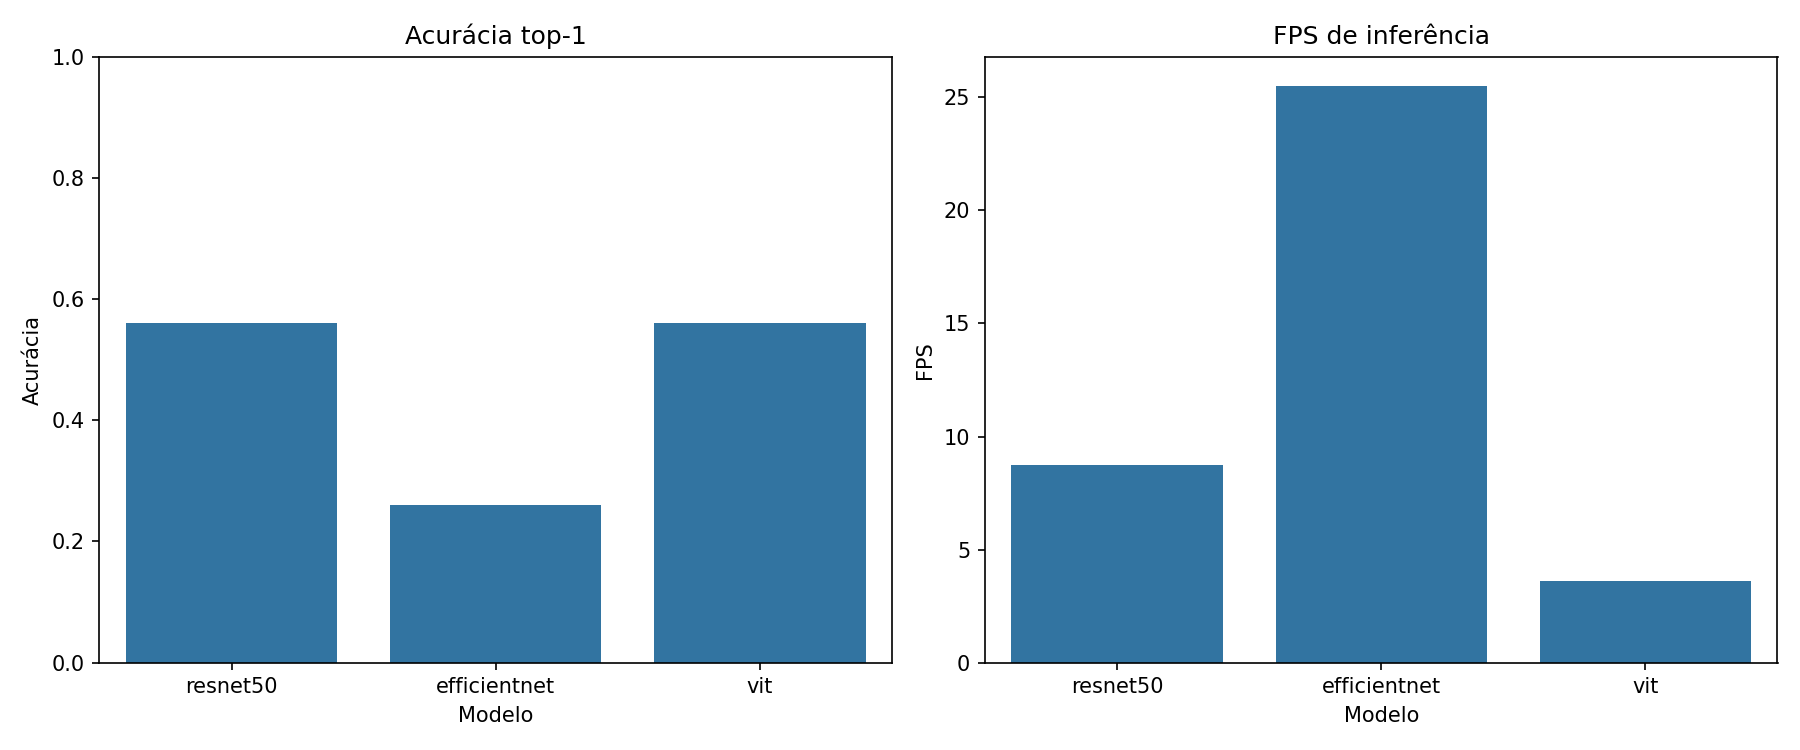
\includegraphics[width=\textwidth,height=0.56\textheight,keepaspectratio]{imagens/accuracy_vs_fps.png}\\
            {\scriptsize\color{muted} EfficientNet isola o FPS.\\ResNet e ViT empatam no acerto.}
        \end{column}
        \begin{column}{0.49\textwidth}
            \centering
            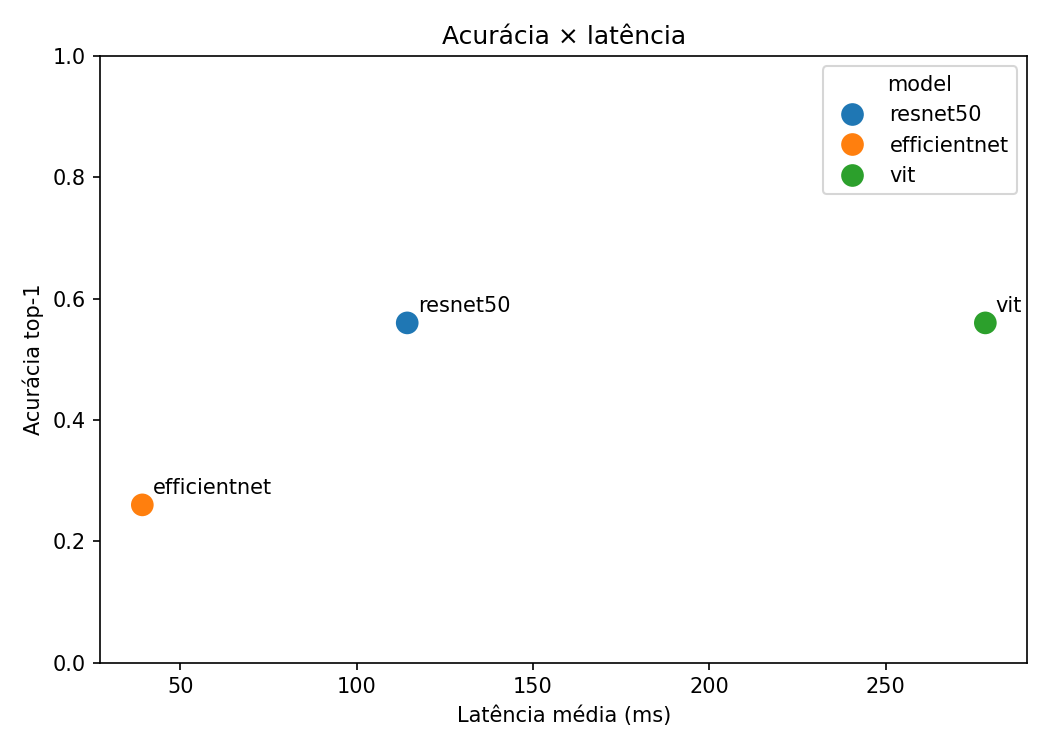
\includegraphics[width=\textwidth,height=0.56\textheight,keepaspectratio]{imagens/accuracy_vs_latency.png}\\
            {\scriptsize\color{muted} O ideal seria o alto à esquerda.\\O ViT paga 56\% com mais espera.}
        \end{column}
    \end{columns}
\end{frame}

\begin{frame}{Os erros têm forma}
    \begin{center}
    \begin{tikzpicture}
        \fill[bad!12, rounded corners=10pt] (0,2.25) rectangle (6.0,4.45);
        \node[align=left, anchor=west, text width=5.4cm] at (0.3,3.35)
            {\textcolor{bad}{\textbf{Teclado na borda}}\\ a ResNet responde \texttt{space bar}};

        \fill[mid!18, rounded corners=10pt] (6.3,2.25) rectangle (12.3,4.45);
        \node[align=left, anchor=west, text width=5.4cm] at (6.6,3.35)
            {\textcolor{mid}{\textbf{Mochila sem alça}}\\ vira \texttt{mailbag} ou colete};

        \fill[vit!12, rounded corners=10pt] (0,0) rectangle (6.0,2.0);
        \node[align=left, anchor=west, text width=5.4cm] at (0.3,1.0)
            {\textcolor{vit}{\textbf{Dois objetos}}\\ a garrafa pode vencer a mochila};

        \fill[ink!8, rounded corners=10pt] (6.3,0) rectangle (12.3,2.0);
        \node[align=left, anchor=west, text width=5.4cm] at (6.6,1.0)
            {\textbf{96\% e ainda errou}\\ o ViT chamou a garrafa de \texttt{safe}};
    \end{tikzpicture}
    \end{center}
\end{frame}

\begin{frame}{Na webcam, a ordem não muda}
    \begin{center}
    \begin{tikzpicture}
        \node[anchor=east, font=\bfseries] at (2.5,3.2) {EfficientNet};
        \fill[soft, rounded corners=4pt] (2.8,2.85) rectangle (11.6,3.55);
        \fill[efficient, rounded corners=4pt] (2.8,2.85) rectangle (11.2,3.55);
        \node[anchor=west, text=white, font=\bfseries] at (3.0,3.2) {15,2 FPS};

        \node[anchor=east, font=\bfseries] at (2.5,1.9) {ResNet-50};
        \fill[soft, rounded corners=4pt] (2.8,1.55) rectangle (11.6,2.25);
        \fill[resnet, rounded corners=4pt] (2.8,1.55) rectangle (6.15,2.25);
        \node[anchor=west, text=white, font=\bfseries] at (3.0,1.9) {6,1};

        \node[anchor=east, font=\bfseries] at (2.5,0.6) {ViT-B/16};
        \fill[soft, rounded corners=4pt] (2.8,0.25) rectangle (11.6,0.95);
        \fill[vit, rounded corners=4pt] (2.8,0.25) rectangle (4.35,0.95);
        \node[anchor=west, text=white, font=\scriptsize\bfseries] at (3.0,0.6) {2,8};
    \end{tikzpicture}
    \end{center}
    \vspace{-1mm}
    {\color{muted}\small Teclas 1, 2 e 3 trocam o modelo na mesma sessão.\\
    O FPS inclui captura e desenho. p95: 51 ms, 168 ms e 342 ms.}
\end{frame}

\begin{frame}{Levar um modelo para casa}
    \begin{center}
    \begin{tikzpicture}
        \fill[resnet] (0,0.4) rectangle (4.0,4.3);
        \node[text=white, align=center, text width=3.5cm] at (2.0,2.35)
            {\textbf{Equilíbrio}\\[6pt]\large ResNet-50\\[4pt]\scriptsize melhor top-5\\e custo do meio};

        \fill[vit] (4.25,0.4) rectangle (8.25,4.3);
        \node[text=white, align=center, text width=3.5cm] at (6.25,2.35)
            {\textbf{Detalhe}\\[6pt]\large ViT-B/16\\[4pt]\scriptsize teclado e garrafa,\\se o tempo permitir};

        \fill[efficient] (8.5,0.4) rectangle (12.5,4.3);
        \node[text=white, align=center, text width=3.5cm] at (10.5,2.35)
            {\textbf{Fluidez}\\[6pt]\large EfficientNet\\[4pt]\scriptsize quando o quadro\\não pode esperar};
    \end{tikzpicture}
    \end{center}
    \vspace{-1mm}
    {\color{muted}\small Limite desta amostra: 50 rótulos, 1 vídeo, 1 classe por quadro e nenhuma GPU.}
\end{frame}

\begin{frame}{O que fica}
    \begin{center}
    \begin{tikzpicture}
        \node[align=center, text=ink, font=\LARGE\bfseries] at (6.2,3.15) {Mesma acurácia, custos diferentes.};
        \fill[resnet, rounded corners=8pt] (0.2,0.35) rectangle (4.0,2.15);
        \node[text=white, align=center] at (2.1,1.25) {\Large\bfseries 88\%\\[1pt]\scriptsize melhor top-5};
        \fill[efficient, rounded corners=8pt] (4.3,0.35) rectangle (8.1,2.15);
        \node[text=white, align=center] at (6.2,1.25) {\Large\bfseries 7\(\times\)\\[1pt]\scriptsize EfficientNet mais\\rápido que o ViT};
        \fill[vit, rounded corners=8pt] (8.4,0.35) rectangle (12.2,2.15);
        \node[text=white, align=center] at (10.3,1.25) {\Large\bfseries 3 objetos\\[1pt]\scriptsize o próximo passo\\é localizar cada um};
    \end{tikzpicture}
    \end{center}
    \vspace{-1mm}
    {\color{muted}\small Cada rede usa a transformação oficial do próprio peso.}
\end{frame}

\begin{frame}{Referências}
    \small
    \begin{tabular}{@{}p{2.4cm}p{9.2cm}@{}}
        \textcolor{resnet}{\textbf{ResNet}} & He, Zhang, Ren e Sun. CVPR, 2016. \\[6pt]
        \textcolor{efficient}{\textbf{EfficientNet}} & Tan e Le. ICML, 2019. \\[6pt]
        \textcolor{vit}{\textbf{ViT}} & Dosovitskiy et al. ICLR, 2021. \\[6pt]
        \textcolor{ink}{\textbf{ImageNet}} & Russakovsky et al. IJCV, 2015.
    \end{tabular}
\end{frame}

\end{document}
